\RequirePackage{currfile}
\documentclass[11pt]{article}
\usepackage[utf8]{inputenc}
\usepackage[ngerman]{babel}
\usepackage{libertine}
\usepackage[a4paper]{geometry}
\usepackage{parskip}
\usepackage{amsmath, amsthm, amssymb} 
\usepackage{mathtools}
\usepackage{booktabs}
\usepackage{tabularx}
\usepackage{enumitem}
\usepackage{graphicx}
\usepackage{xcolor}
\usepackage{float}
\usepackage{wrapfig}
\usepackage[makeroom]{cancel}
\usepackage{multicol}
\usepackage{multirow}
\usepackage{vwcol} 	 	% Provides variable multicol
\usepackage{commath} 	% Provides good differentials
\usepackage{esint} 		% Provides various fancy integral symbols
\usepackage{siunitx} 	% Provides good units
\usepackage{nicefrac}
\usepackage{dashrule}
\usepackage{minted}

\usepackage[version=0.96]{pgf}
\usepackage{tikz}
\usetikzlibrary{arrows,shapes,snakes,automata,backgrounds,petri,positioning}

\usepackage{csquotes}
\MakeOuterQuote{"}

% http://packages.oth-regensburg.de/ctan/macros/latex/contrib/currfile/currfile.pdf
% % https://tex.stackexchange.com/a/54891/116525

\makeatletter
\newcommand{\toleftmargin}[1]{\par\noindent\hspace{-\@totalleftmargin}\parbox[t]{\textwidth}{#1}}
% \newenvironment{javaenv}{\begin{minted}[linenos,firstnumber=last,autogobble,xleftmargin=-\@totalleftmargin]{java}}{}
\newlength{\leftmargins}
\makeatother
% https://tex.stackexchange.com/a/481735

\def\nrub{7}
\newcommand{\blanko}[0]{\textcolor{white}{.}}

\usepackage{hyperref}
\hypersetup{
	pdftitle={Betriebsysteme (WS19/20) Übungsblatt \nrub ~- 12141043},
	pdfauthor={Yudong SUn},
	bookmarksnumbered=true,
	bookmarksopen=true,
	bookmarksopenlevel=2,
	pdfstartview=Fit,
	pdfpagemode=UseOutlines,
	colorlinks=true,
	linkcolor=black,
	filecolor=magenta,      
	urlcolor=blue
}
\urlstyle{same}

\renewcommand{\ttdefault}{cmtt}

\usepackage{fancyhdr}
 
\pagestyle{fancy}
\fancyhf{}
\fancyhead[RO]{Yudong Sun / \texttt{12141043}}
\fancyhead[LO]{Übungsblatt \nrub}
\fancyhead[LE]{\texttt{12141043} / Yudong Sun}
\fancyhead[RE]{Übungsblatt \nrub}
\cfoot{\thepage}

\title{Betriebsysteme (WS19/20)\\Übungsblatt \nrub}
\author{Yudong Sun\\\texttt{12141043}}
\date{\today}

\begin{document}

\maketitle

% \begin{enumerate}[label={T\arabic*},start=2]
	\item 
\end{enumerate}

koelle.michael"campus.lmu.de
Klausur 6.2.2020 1830 2030
Einsicht: 18.2.2020

Aufgabe 5.txt -> 
a) 
ib) iii

@remote.cip.ifl.lmu.de
ab Windows 10 1809 integriert


====

SPIM
what i dont understand: syscalls
dereferencing

===

\begin{enumerate}[label={Aufgabe H\arabic*},start=31]
    \item Sie können den Quellcode auch in der Datei \texttt{Server.java.txt} sehen.
        \begin{enumerate}
            \makeatletter
                \setlength{\leftmargins}{\@totalleftmargin}
            \makeatother

            \item \blanko
                \begin{minted}[linenos,firstnumber=7,autogobble,xleftmargin=-\leftmargins,frame=leftline,framesep=10pt]{java}
                    public Server(int maxClients)
                    {
                        this.maxClients = maxClients;
                        this.anzahlClients = 0;
                        this.sicherungswunsch = false;
                    }
                \end{minted}
            \item \blanko 

                \begin{minted}[linenos,firstnumber=last,autogobble,xleftmargin=-\leftmargins,frame=leftline,framesep=10pt]{java}
                    public synchronized void daten_ablegen(Client c) throws InterruptedException
                    {
                        System.out.println("Client " + c.ID + " will Daten ablegen");
                        
                    // ----- kritischer Bereich -----
                        while(this.anzahlClients >= this.maxClients || this.sicherungswunsch)
                        {
                            try { wait(); }
                            catch(InterruptedException e) {} // <<<<<< nicht nötig
                        }
                        anzahlClients ++; 
                        System.out.println(anzahlClients + " Clients legen Daten ab.");
                    }
                    public synchronized void daten_ablegen_beenden()
                    {
                        anzahlClients --;
                    // ----- kritischer Bereich verlassen -----
                        notifyAll(); // Mehrere Prozesse -> notifyAll() statt notify()
                    } 
                \end{minted}

                Es gibt bei beider Methoden kein "Sanity Check", da wir davon ausgehen, dass die Methoden immer in einer sinnvollen Reihenfolge aufgerufen werden.
            \item \blanko

                \begin{minted}[linenos,firstnumber=last,autogobble,xleftmargin=-\leftmargins,frame=leftline,framesep=10pt]{java}
                    public synchronized void sicherungAktivieren() throws InterruptedException
                    {
                        this.sicherungswunsch = true;
                        System.out.println("Sicherungswunsch angemeldet!");
                
                        notifyAll();    // << Nicht nötig, nur für wait()
                        
                    // ----- kritischer Bereich -----
                        while(this.anzahlClients > 0)
                        {
                            try { wait(); }
                            catch(InterruptedException e) {}
                        }
                        // Zum Sichern bereit.
                    }   
                    public synchronized void sicherungDeaktivieren()
                    {
                        this.sicherungswunsch = false;
                    // ----- kritischer Bereich verlassen -----
                        System.out.println("Sicherungswunsch deaktiviert.");
                        notifyAll();
                    }
                \end{minted}
            \item Die 2 kritische Bereichen sind:
                \begin{itemize}
                    \item Als ein Client Daten in den Server ablegen möchte, und
                    \item Als das Sicherungsskript eine Sicherung machen möchte.
                \end{itemize}

                % Setzen von sicherungswunsch
                % Inkrementieren/Dekrementieren von anzahlClients

                % Mutual Exclusion durch das Schluesselwort synchronized in der Methodendeklaration

                Die beide Bereichen beziehen sich auf das Schreiben bzw. Lesen von Daten. Es wird hier mithilfe der folgenden Schritten sichergestellt, dass die Bedingungen der wechseitiges Anschluss erfüllt ist:
                \begin{itemize}
                    \item Die Methoden sind alle synchronisiert. 
                    \item Die Betriebstatus des Systems wird durch die Variablen \mintinline{java}{Server.anzahlClients} und \mintinline{java}{Server.sicherungswunsch} gespeichert. Sie werden bei jedem Methodenaufruf aktualisiert.
                    \item Das Sicherungsskript wartet darauf, dass \mintinline{java}{Server.anzahlClients} null ist. Das stellt es sicher, dass kein Client legt Daten auf dem Server.
                    \item Die Clients warten, wenn \mintinline{java}{Server.sicherungswunsch} wahr ist. 

                    \mintinline{java}{Server.sicherungswunsch} wird nur wieder auf falsch gestellt, wenn das Sicherungsskript fertig ist. Das stellt es sicher, dass kein Client legt mehr Daten auf dem Server, wenn eine Sicherung durchgeführt wird. 
                \end{itemize}

                Dabei entsteht wechselseitige Ausschluss.
        \end{enumerate}
    \item Alle Stellen haben die Kapazität $\infty$ und alle Kanten haben das Gewicht 1. Die Stellen für die Semphoren exisiert nur, weil die Kanten alle das Gewicht 1 haben müssen. Die Anfangsmarkierung beschreibt die in dem Übungsblatt gezeichneten Situation:

        \vspace{2em}

        \begin{figure}[h!]
            \centering
            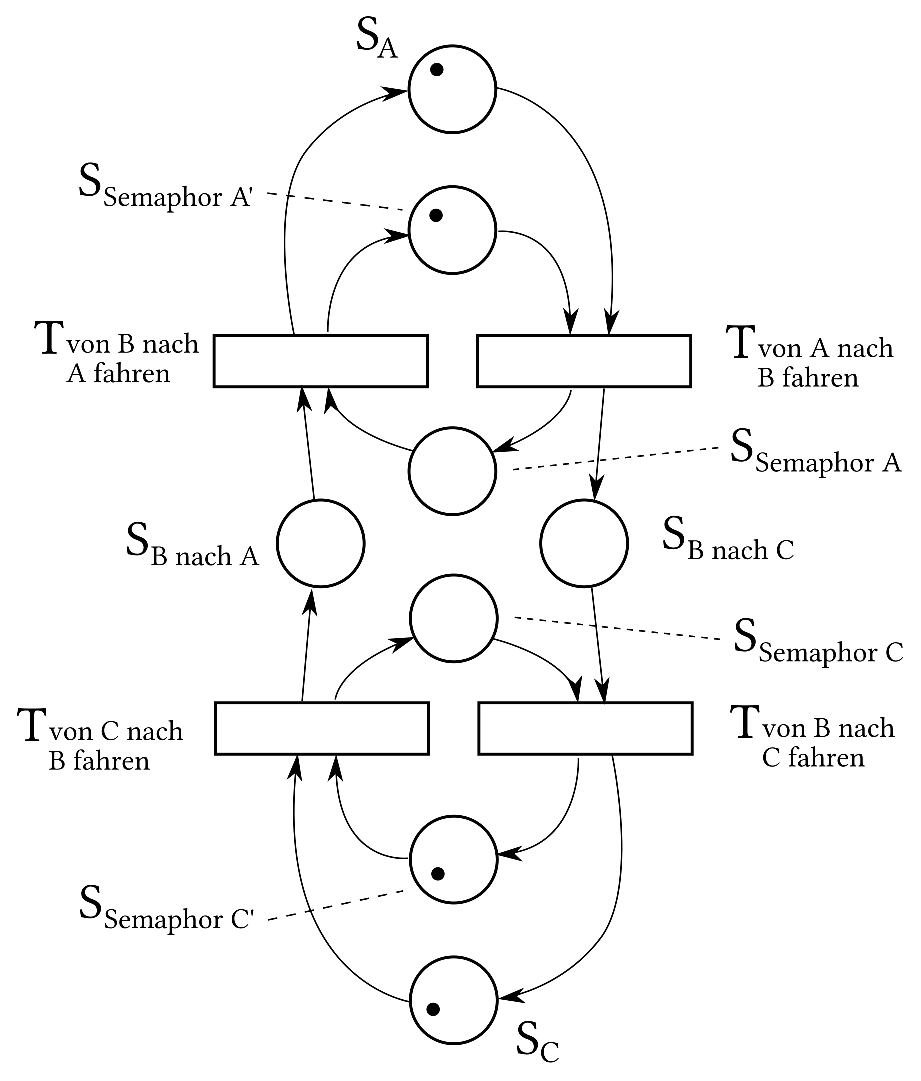
\includegraphics[width=0.7\textwidth]{q32.eps}
            \caption{Petri-Netz Aufgabe 32}

            LOL OKAY THERE IS NO CONSERVATION OF MARKE Semaphor A' bzw. C' nicht nötig
        \end{figure}

        Es gibt 2 Stellen für den Abschnitt B, um die Bedingungung zu modellieren, dass kein Richtungswechsel in B möglich ist. Die Sicherheitsbedingung wird durch die Semaphoren $S_{\text{Semaphor } A}$ und $S_{\text{Semaphor } C}$ bzw. $S_{\text{Semaphor } A'}$ und $S_{\text{Semaphor } C'}$ sicher gestellt. 
    \item Sehen Sie bitte \texttt{u06-h33.txt}
\end{enumerate}


\end{document}
